% Created by tikzDevice version 0.12
% !TEX encoding = UTF-8 Unicode
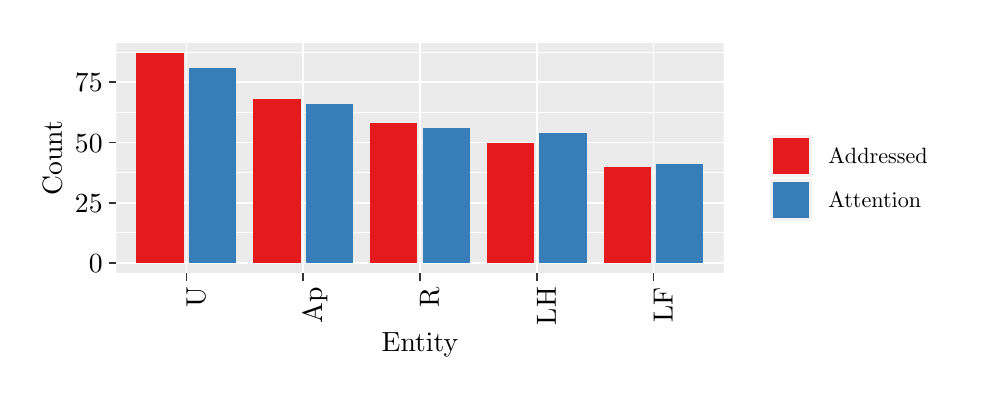
\begin{tikzpicture}[x=1pt,y=1pt]
\definecolor{fillColor}{RGB}{255,255,255}
\path[use as bounding box,fill=fillColor,fill opacity=0.00] (0,0) rectangle (336.00,124.59);
\begin{scope}
\path[clip] (  0.00,  0.00) rectangle (336.00,124.59);
\definecolor{drawColor}{RGB}{255,255,255}
\definecolor{fillColor}{RGB}{255,255,255}

\path[draw=drawColor,line width= 0.6pt,line join=round,line cap=round,fill=fillColor] (  0.00,  0.00) rectangle (336.00,124.59);
\end{scope}
\begin{scope}
\path[clip] ( 32.03, 35.78) rectangle (251.44,119.09);
\definecolor{fillColor}{gray}{0.92}

\path[fill=fillColor] ( 32.03, 35.78) rectangle (251.44,119.09);
\definecolor{drawColor}{RGB}{255,255,255}

\path[draw=drawColor,line width= 0.3pt,line join=round] ( 32.03, 50.45) --
	(251.44, 50.45);

\path[draw=drawColor,line width= 0.3pt,line join=round] ( 32.03, 72.21) --
	(251.44, 72.21);

\path[draw=drawColor,line width= 0.3pt,line join=round] ( 32.03, 93.97) --
	(251.44, 93.97);

\path[draw=drawColor,line width= 0.3pt,line join=round] ( 32.03,115.74) --
	(251.44,115.74);

\path[draw=drawColor,line width= 0.6pt,line join=round] ( 32.03, 39.56) --
	(251.44, 39.56);

\path[draw=drawColor,line width= 0.6pt,line join=round] ( 32.03, 61.33) --
	(251.44, 61.33);

\path[draw=drawColor,line width= 0.6pt,line join=round] ( 32.03, 83.09) --
	(251.44, 83.09);

\path[draw=drawColor,line width= 0.6pt,line join=round] ( 32.03,104.86) --
	(251.44,104.86);

\path[draw=drawColor,line width= 0.6pt,line join=round] ( 57.35, 35.78) --
	( 57.35,119.09);

\path[draw=drawColor,line width= 0.6pt,line join=round] ( 99.54, 35.78) --
	( 99.54,119.09);

\path[draw=drawColor,line width= 0.6pt,line join=round] (141.74, 35.78) --
	(141.74,119.09);

\path[draw=drawColor,line width= 0.6pt,line join=round] (183.93, 35.78) --
	(183.93,119.09);

\path[draw=drawColor,line width= 0.6pt,line join=round] (226.13, 35.78) --
	(226.13,119.09);
\definecolor{fillColor}{RGB}{228,26,28}

\path[fill=fillColor] ( 39.31, 39.56) rectangle ( 56.40,115.30);
\definecolor{fillColor}{RGB}{55,126,184}

\path[fill=fillColor] ( 58.30, 39.56) rectangle ( 75.38,110.08);
\definecolor{fillColor}{RGB}{228,26,28}

\path[fill=fillColor] ( 81.50, 39.56) rectangle ( 98.59, 98.76);
\definecolor{fillColor}{RGB}{55,126,184}

\path[fill=fillColor] (100.49, 39.56) rectangle (117.58, 97.02);
\definecolor{fillColor}{RGB}{228,26,28}

\path[fill=fillColor] (123.70, 39.56) rectangle (140.79, 90.06);
\definecolor{fillColor}{RGB}{55,126,184}

\path[fill=fillColor] (142.69, 39.56) rectangle (159.77, 88.32);
\definecolor{fillColor}{RGB}{228,26,28}

\path[fill=fillColor] (165.89, 39.56) rectangle (182.98, 83.09);
\definecolor{fillColor}{RGB}{55,126,184}

\path[fill=fillColor] (184.88, 39.56) rectangle (201.97, 86.57);
\definecolor{fillColor}{RGB}{228,26,28}

\path[fill=fillColor] (208.09, 39.56) rectangle (225.18, 74.39);
\definecolor{fillColor}{RGB}{55,126,184}

\path[fill=fillColor] (227.07, 39.56) rectangle (244.16, 75.26);
\end{scope}
\begin{scope}
\path[clip] (  0.00,  0.00) rectangle (336.00,124.59);
\definecolor{drawColor}{RGB}{0,0,0}

\node[text=drawColor,anchor=base east,inner sep=0pt, outer sep=0pt, scale=  1.00] at ( 27.08, 36.12) {0};

\node[text=drawColor,anchor=base east,inner sep=0pt, outer sep=0pt, scale=  1.00] at ( 27.08, 57.88) {25};

\node[text=drawColor,anchor=base east,inner sep=0pt, outer sep=0pt, scale=  1.00] at ( 27.08, 79.65) {50};

\node[text=drawColor,anchor=base east,inner sep=0pt, outer sep=0pt, scale=  1.00] at ( 27.08,101.41) {75};
\end{scope}
\begin{scope}
\path[clip] (  0.00,  0.00) rectangle (336.00,124.59);
\definecolor{drawColor}{gray}{0.20}

\path[draw=drawColor,line width= 0.6pt,line join=round] ( 29.28, 39.56) --
	( 32.03, 39.56);

\path[draw=drawColor,line width= 0.6pt,line join=round] ( 29.28, 61.33) --
	( 32.03, 61.33);

\path[draw=drawColor,line width= 0.6pt,line join=round] ( 29.28, 83.09) --
	( 32.03, 83.09);

\path[draw=drawColor,line width= 0.6pt,line join=round] ( 29.28,104.86) --
	( 32.03,104.86);
\end{scope}
\begin{scope}
\path[clip] (  0.00,  0.00) rectangle (336.00,124.59);
\definecolor{drawColor}{gray}{0.20}

\path[draw=drawColor,line width= 0.6pt,line join=round] ( 57.35, 33.03) --
	( 57.35, 35.78);

\path[draw=drawColor,line width= 0.6pt,line join=round] ( 99.54, 33.03) --
	( 99.54, 35.78);

\path[draw=drawColor,line width= 0.6pt,line join=round] (141.74, 33.03) --
	(141.74, 35.78);

\path[draw=drawColor,line width= 0.6pt,line join=round] (183.93, 33.03) --
	(183.93, 35.78);

\path[draw=drawColor,line width= 0.6pt,line join=round] (226.13, 33.03) --
	(226.13, 35.78);
\end{scope}
\begin{scope}
\path[clip] (  0.00,  0.00) rectangle (336.00,124.59);
\definecolor{drawColor}{RGB}{0,0,0}

\node[text=drawColor,rotate= 90.00,anchor=base east,inner sep=0pt, outer sep=0pt, scale=  1.00] at ( 64.23, 30.83) {U};

\node[text=drawColor,rotate= 90.00,anchor=base east,inner sep=0pt, outer sep=0pt, scale=  1.00] at (106.43, 30.83) {Ap};

\node[text=drawColor,rotate= 90.00,anchor=base east,inner sep=0pt, outer sep=0pt, scale=  1.00] at (148.62, 30.83) {R};

\node[text=drawColor,rotate= 90.00,anchor=base east,inner sep=0pt, outer sep=0pt, scale=  1.00] at (190.82, 30.83) {LH};

\node[text=drawColor,rotate= 90.00,anchor=base east,inner sep=0pt, outer sep=0pt, scale=  1.00] at (233.01, 30.83) {LF};
\end{scope}
\begin{scope}
\path[clip] (  0.00,  0.00) rectangle (336.00,124.59);
\definecolor{drawColor}{RGB}{0,0,0}

\node[text=drawColor,anchor=base,inner sep=0pt, outer sep=0pt, scale=  1.00] at (141.74,  7.44) {Entity};
\end{scope}
\begin{scope}
\path[clip] (  0.00,  0.00) rectangle (336.00,124.59);
\definecolor{drawColor}{RGB}{0,0,0}

\node[text=drawColor,rotate= 90.00,anchor=base,inner sep=0pt, outer sep=0pt, scale=  1.00] at ( 12.39, 77.43) {Count};
\end{scope}
\begin{scope}
\path[clip] (  0.00,  0.00) rectangle (336.00,124.59);
\definecolor{fillColor}{RGB}{255,255,255}

\path[fill=fillColor] (262.44, 48.87) rectangle (330.50,106.00);
\end{scope}
\begin{scope}
\path[clip] (  0.00,  0.00) rectangle (336.00,124.59);
\definecolor{drawColor}{RGB}{255,255,255}
\definecolor{fillColor}{gray}{0.95}

\path[draw=drawColor,line width= 0.6pt,line join=round,line cap=round,fill=fillColor] (267.94, 70.27) rectangle (283.84, 86.17);
\end{scope}
\begin{scope}
\path[clip] (  0.00,  0.00) rectangle (336.00,124.59);
\definecolor{fillColor}{RGB}{228,26,28}

\path[fill=fillColor] (269.37, 71.69) rectangle (282.42, 84.74);
\end{scope}
\begin{scope}
\path[clip] (  0.00,  0.00) rectangle (336.00,124.59);
\definecolor{drawColor}{RGB}{255,255,255}
\definecolor{fillColor}{gray}{0.95}

\path[draw=drawColor,line width= 0.6pt,line join=round,line cap=round,fill=fillColor] (267.94, 54.37) rectangle (283.84, 70.27);
\end{scope}
\begin{scope}
\path[clip] (  0.00,  0.00) rectangle (336.00,124.59);
\definecolor{fillColor}{RGB}{55,126,184}

\path[fill=fillColor] (269.37, 55.79) rectangle (282.42, 68.85);
\end{scope}
\begin{scope}
\path[clip] (  0.00,  0.00) rectangle (336.00,124.59);
\definecolor{drawColor}{RGB}{0,0,0}

\node[text=drawColor,anchor=base west,inner sep=0pt, outer sep=0pt, scale=  0.80] at (289.34, 75.46) {Addressed};
\end{scope}
\begin{scope}
\path[clip] (  0.00,  0.00) rectangle (336.00,124.59);
\definecolor{drawColor}{RGB}{0,0,0}

\node[text=drawColor,anchor=base west,inner sep=0pt, outer sep=0pt, scale=  0.80] at (289.34, 59.56) {Attention};
\end{scope}
\end{tikzpicture}
